%!TEX program = xelatex
\documentclass[xcolor={table}]{beamer}

\usepackage[brazil]{babel}	
\usepackage[utf8]{inputenc}
\usepackage[T1]{fontenc}
\usepackage[scaled]{helvet}
\usepackage{amsthm}
\usepackage{ragged2e}
\usepackage{subfig}
\usepackage[table]{xcolor}
\usepackage{multicol}
\usepackage{multirow}
\usepackage{fancyvrb}
\usepackage{verbatim}
\usepackage{hyperref}
\definecolor{gold}{rgb}{0.81,0.69,0}
\definecolor{silver}{rgb}{0.75,0.75,0.75}
\usetheme{Execushares}

\title{Laborator 3 - GPIO}
\subtitle{}
\author{Coca Mihai \\
        Ioana Dragoș}

\setcounter{showSlideNumbers}{1}

\begin{document}
	\setcounter{showProgressBar}{0}
	\setcounter{showSlideNumbers}{0}

	\frame{\titlepage}

	\begin{frame}
		\frametitle{Tabelă de Conținut}
		\begin{enumerate}
            \item Concepte teoretice
			\item Electronică de bază
			\item Configurare
			\item Exemplu practic
		\end{enumerate}
	\end{frame}

	\setcounter{framenumber}{0}
	\setcounter{showProgressBar}{1}
	\setcounter{showSlideNumbers}{1}
	\section{Concepte teoretice}
	\begin{frame}
	    \frametitle{GPIO}
	    \begin{itemize}
	        \item \textbf{\textit{General Purpose Input/Output}}
	        \item Permite controlarea la run-time a comportamentului unui pin al unui circuit integrat, mai specific, a direcției de trecere a curentului electric prin el și valoarea logică pe care acesta o are
	        \item Un pin poate fi configurat pentru \textbf{\textit{scriere}} sau \textbf{\textit{citire}}
	        \item \textbf{\textit{Interfațare}} (dispozitive externe):
	        \begin{itemize}
	            \item \textbf{\textit{Intrare}} - switch
	            \item \textbf{\textit{Ieșire}} - LED
	        \end{itemize}
	        
	        
	    \end{itemize}
	\end{frame}
		\begin{frame}
	    \frametitle{Noțiuni introductive}
	    \begin{itemize}
	        \item \textbf{\textit{GPIO FRDM-KL25Z}}
	        \begin{itemize}
	            \item \textbf{\textit{PortA (PTA)}}  - pinii 0-5, 12-20
	            \item \textbf{\textit{PortB (PTB)}}  - pinii 0-3, 8-11, 16-19
	            \item \textbf{\textit{PortC (PTC)}}  - pinii 0-13, 16-17
	            \item \textbf{\textit{PortD (PTD)}}  - pinii 0-7
	            \item \textbf{\textit{PortE (PTE)}}  - pinii 0-5, 20-25, 29-31
	            \item \textbf{\textit{Porturile care suportă întreruperi sunt A și D!}}
	        \end{itemize}
	        \item Pentru utilizarea pinilor pentru GPIO este necesară activarea modulului de ceas
	        
	    \end{itemize}
	\end{frame}
	\section{Electronică de bază}
	\begin{frame}
	    \frametitle{Conexiunea pinilor}
	    \begin{itemize}
	        \item O primă variantă de conectare a unui \textbf{switch} cu un pin configurat pentru input GPIO este reprezentat în circuitul următor
	    \end{itemize}
	    \begin{figure}
	        \centering
	        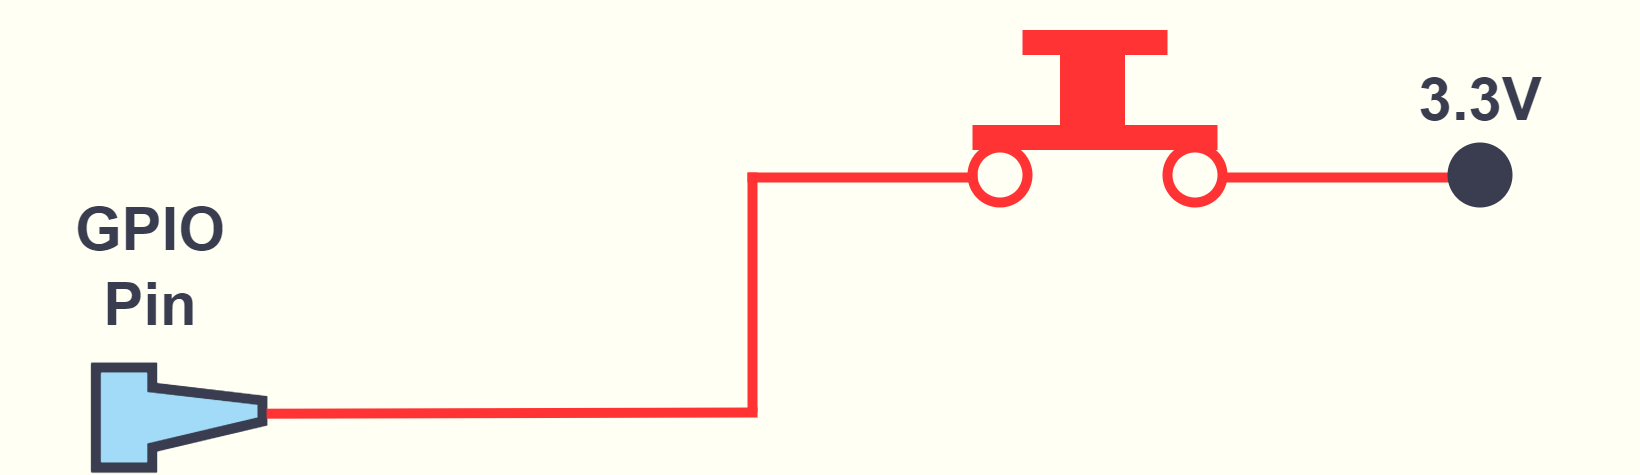
\includegraphics[width=6.5cm]{images/gpio1-onlyvcc-pressed.png}
	        \caption{GPIO Input - VCC \textbf{(Pressed Switch)}}
	        \label{fig:my_label}
	    \end{figure}
	    \begin{itemize}
	        \item Atunci când switch-ul este apăsat, pe pin se va recepționa nivelul 1 logic
	    \end{itemize}
	\end{frame}
		\begin{frame}
	    \frametitle{Conexiunea pinilor}
	    \begin{itemize}
	        \item \textbf{\textit{\color{red}Problemă: }} Când switch-ul este deschis, valoarea recepționată pe pin poartă numele de \textbf{\textit{floating input}}
	        \item \textbf{\textit{Floating input }} - nivelul logic primit pe pin este nedefinit
	        \item \textbf{\textit{Soluție?}}
	    \end{itemize}
	    \begin{figure}
	        \centering
	        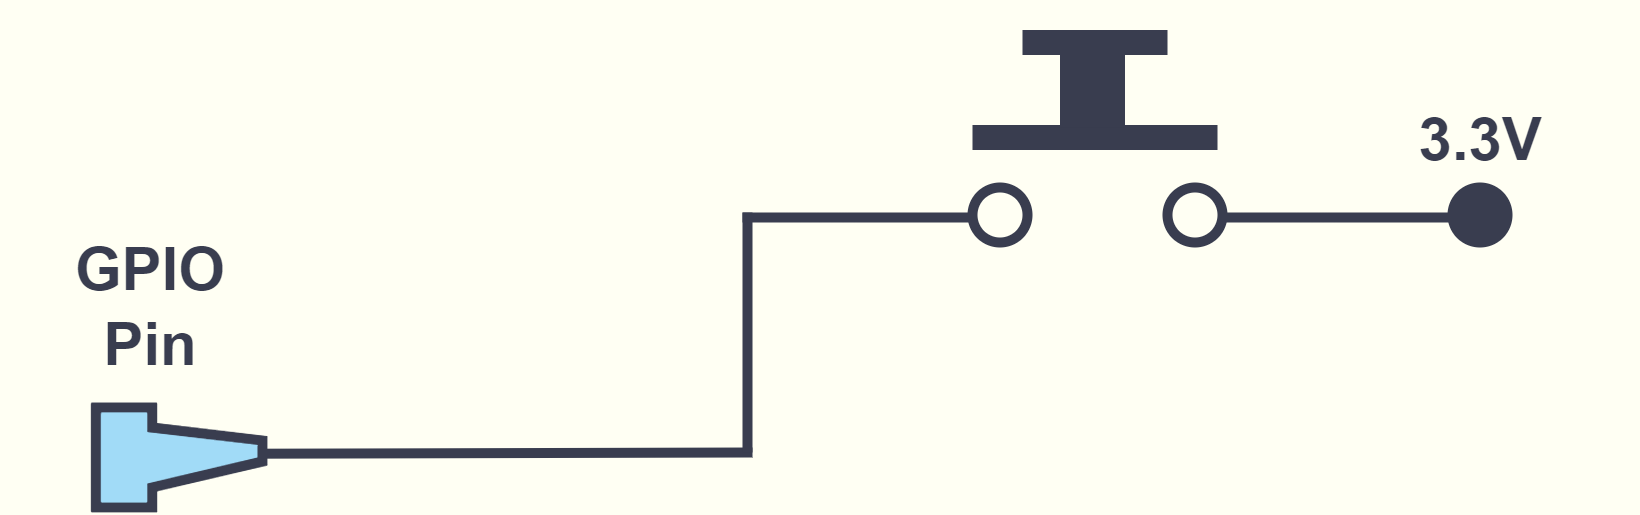
\includegraphics[width=6.5cm]{images/gpio1-onlyvcc-open.png}
	        \caption{GPIO Input - VCC \textbf{(Open Switch)}}
	        \label{fig:my_label}
	    \end{figure}
	\end{frame}
	\begin{frame}
	    \frametitle{Conexiunea pinilor}
	    \begin{itemize}
	        \item Pentru rezolvarea problemei anterioare, putem conecta pinul de \textbf{\textit{GPIO}} la \textbf{\textit{GND}}, astfel încât atunci când switch-ul nu este apăsat, să fie recepționat \textbf{\textit{nivelul logic 0}}.
	    \end{itemize}
	    \begin{figure}
	        \centering
	        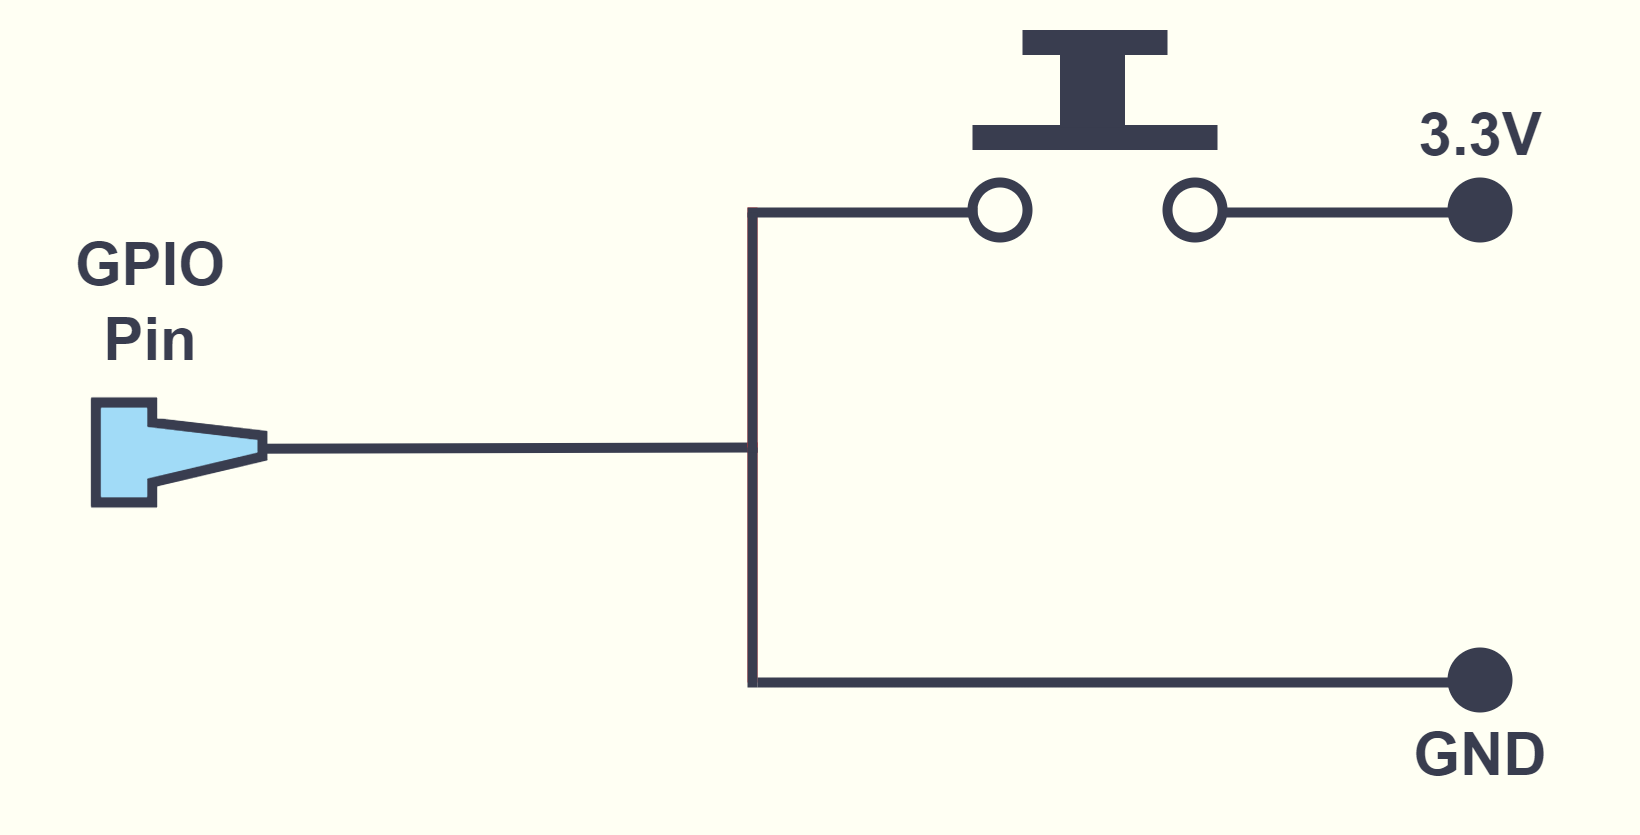
\includegraphics[width=6.5cm]{images/gpio2-vccandgnd-open.png}
	        \caption{GPIO Input - VCC și GND \textbf{(Open Switch)}}
	        \label{fig:my_label}
	    \end{figure}
	\end{frame}
		\begin{frame}
	    \frametitle{Conexiunea pinilor}
	    \begin{itemize}
	        \item \textbf{\textit{\color{red}Problemă: }} Când switch-ul este apăsat, pinul va fi conectat atât la GND, cât și la VCC, producându-se astfel un \textbf{\textit{scurtcircuit}}
	        \item \textbf{\textit{Soluție?}}
	    \end{itemize}
	    \begin{figure}
	        \centering
	        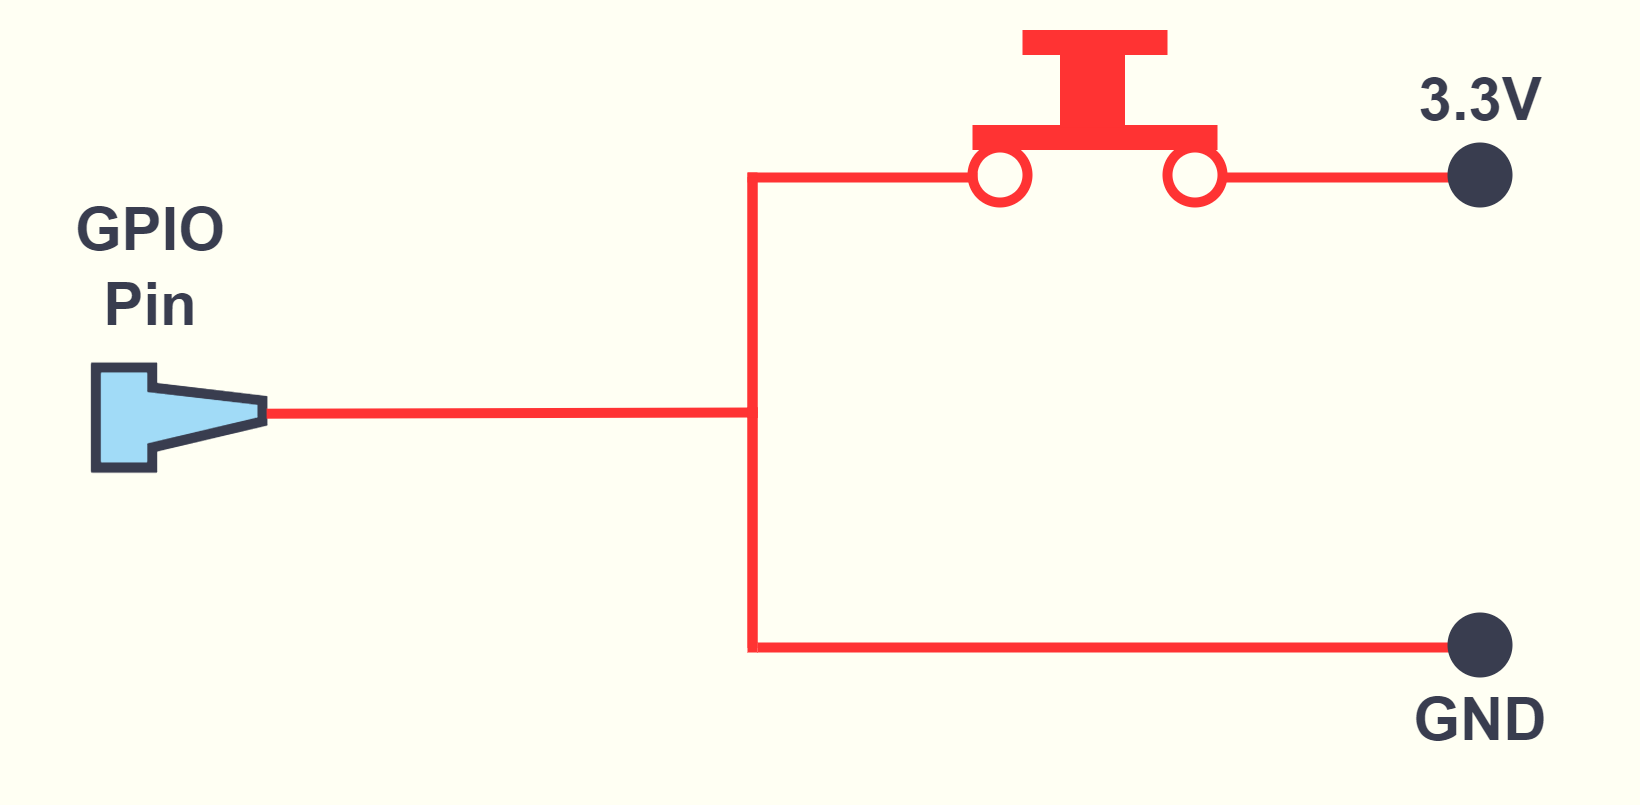
\includegraphics[width=6.5cm]{images/gpio2-vccandgnd-pressed.png}
	        \caption{GPIO Input - VCC și GND \textbf{(Pressed Switch)}}
	        \label{fig:my_label}
	    \end{figure}
	\end{frame}
    \begin{frame}
	    \frametitle{Rezistență de tip pull-down}
	    \begin{itemize}
	        \item Pentru a folosi în practică circuitul anterior, includem o rezistență conectată fie la GND (\textbf{\textit{pull-down}}), fie la VCC (\textbf{\textit{pull-up}}) cu rolul de a defini nivelul logic de pe pinul folosit la GPIO
	    \end{itemize}
	    \begin{figure}
	        \centering
	        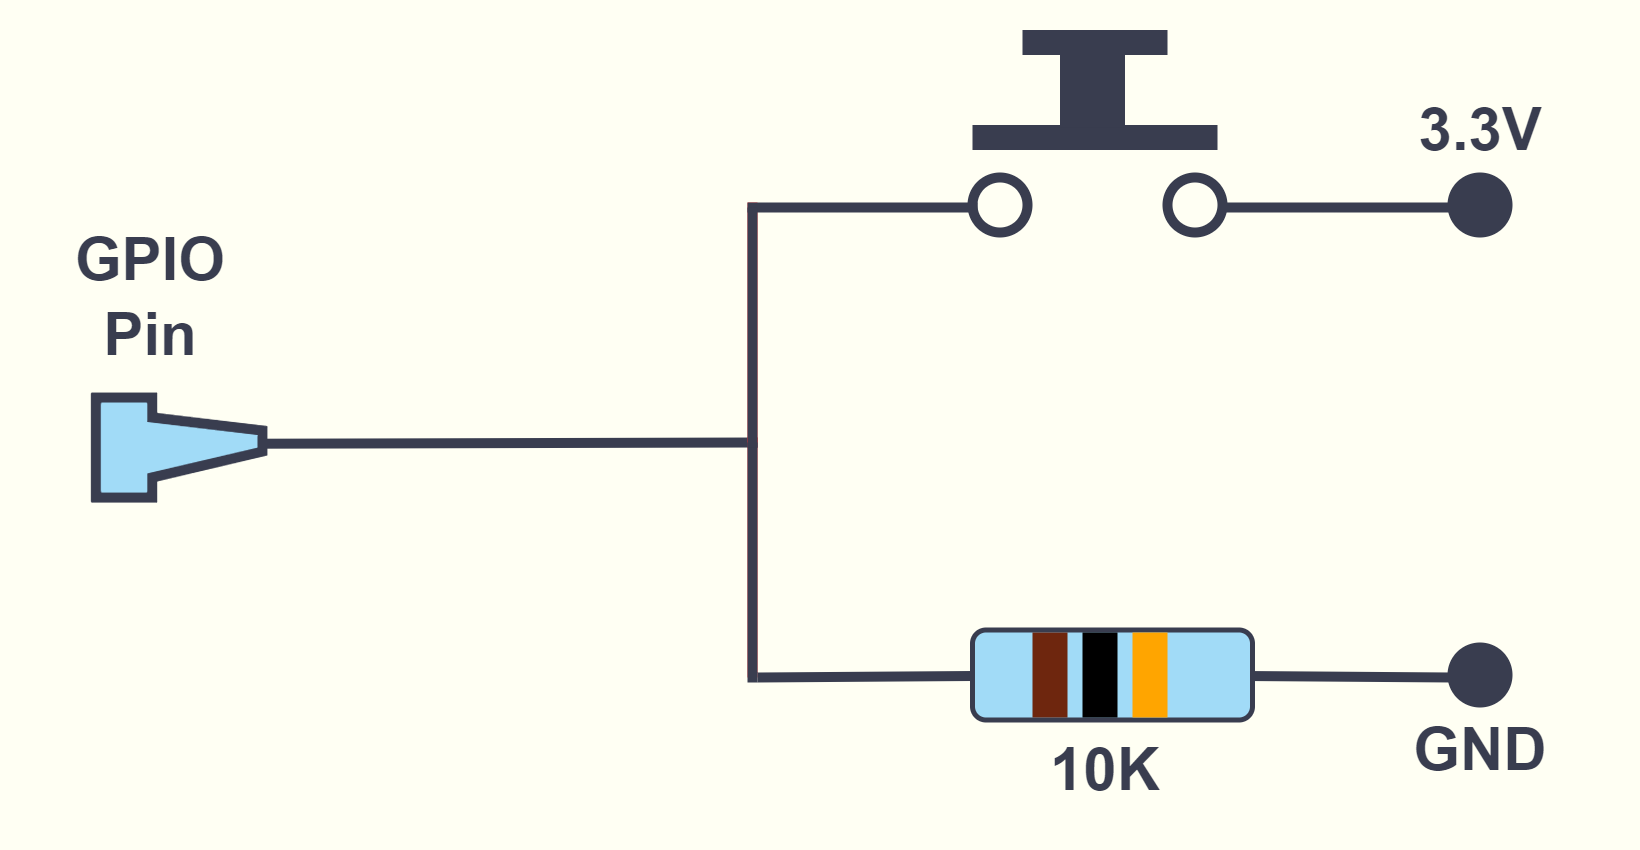
\includegraphics[width=6.5cm]{images/gpio3-pulldown.png}
	        \caption{GPIO Input - Aranjament Pull-down \textbf{(Open Switch)}}
	        \label{fig:my_label}
	    \end{figure}
	\end{frame}
	    \begin{frame}
	    \frametitle{Rezistență de tip pull-up}
	    \begin{itemize}
	        \item Valoarea rezistenței \sim 10 K$\Omega$	  \item \textbf{\textit{Pull-up}} (folosit de regulă în conjuncție cu butoane și switch-uri) - Open high, Pressed low
	        \item \textbf{\textit{Pull-down}} - Open low, Pressed high
	    \end{itemize}
	    \begin{figure}
	        \centering
	        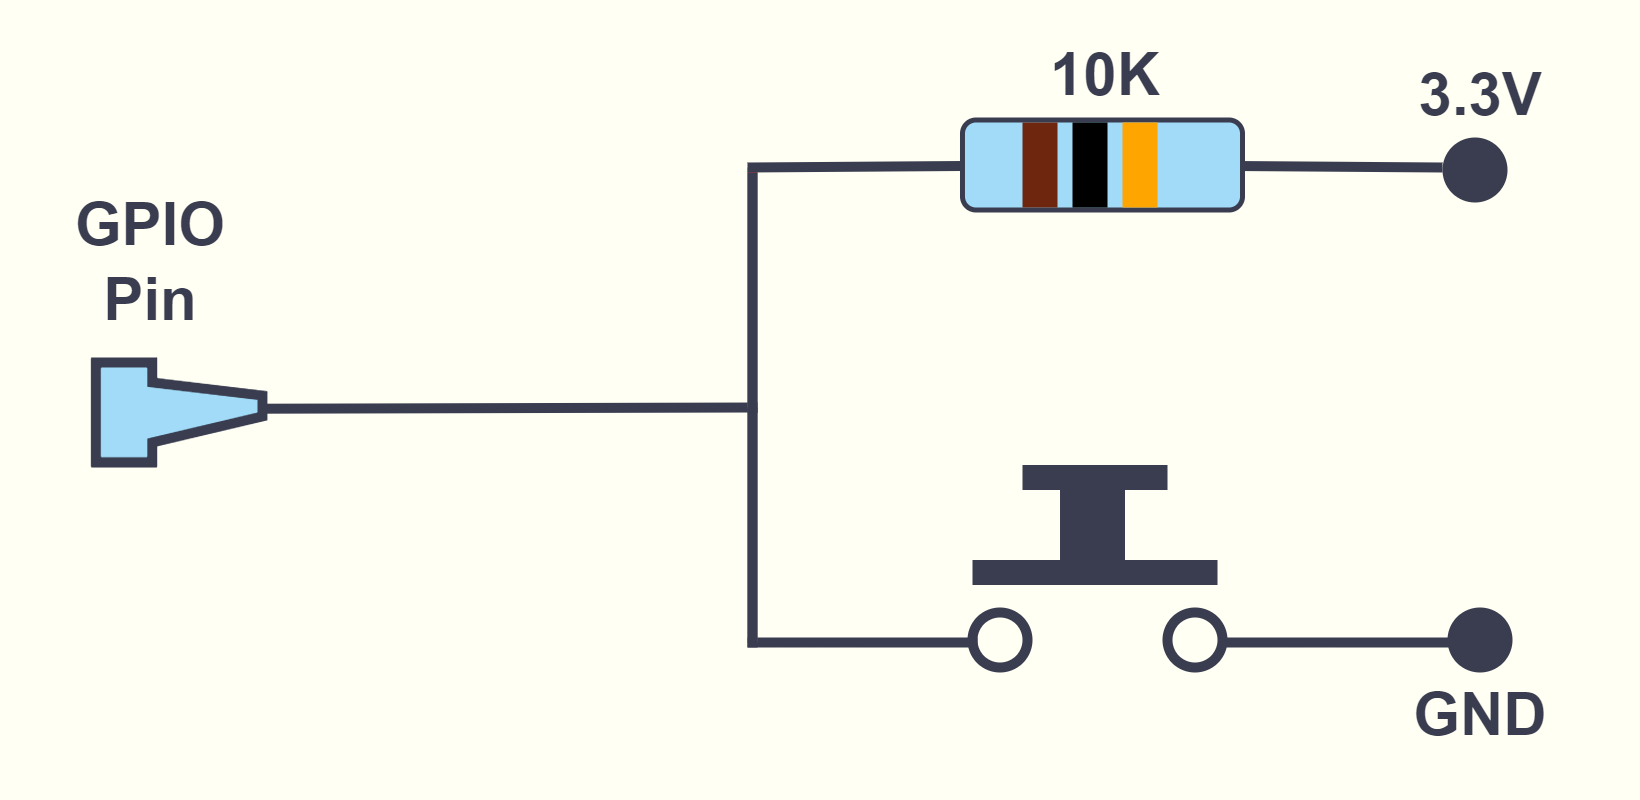
\includegraphics[width=6.5cm]{images/gpio4-pullup.png}
	        \caption{GPIO Input - Aranjament Pull-up \textbf{(Open Switch)}}
	        \label{fig:my_label}
	    \end{figure}
	\end{frame}
	\begin{frame}
	    \frametitle{Aranjament pull-down}
	    \begin{itemize}
	        \item Poate interveni cazul când realizăm o configurare greșită a pinului de GPIO pentru ouput, caz în care putem deteriora plăcuța din cauza nivelului mare de curent care trece prin pin
	        \item \textbf{\textit{Opțional}}: putem adăuga o rezistență cu scopul de limitare a curentului 
	    \end{itemize}
	    \begin{figure}
	        \centering
	        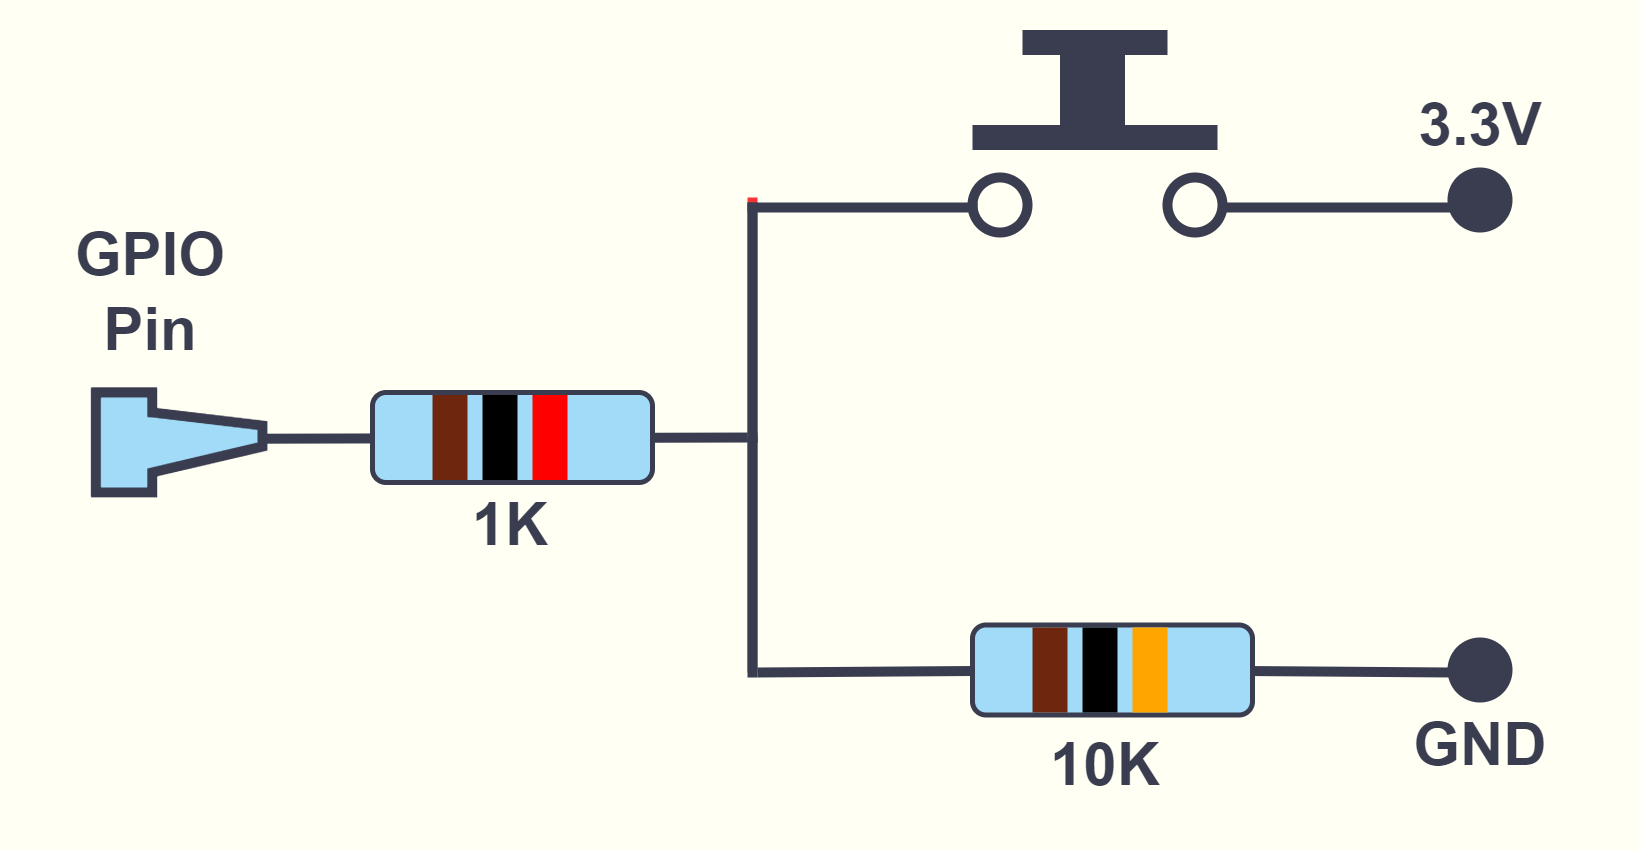
\includegraphics[width=5.5cm]{images/gpio5-limitingresistor.png}
	        \caption{GPIO Input - Aranjament Pull-down cu rezistență de limitare}
	        \label{fig:my_label}
	    \end{figure}
	\end{frame}
		\begin{frame}
	    \frametitle{Schemă circuit electric}
	    \begin{minipage}{0.35\textwidth}
	    \vspace{1cm}
	    \begin{figure}
	        \centering
	        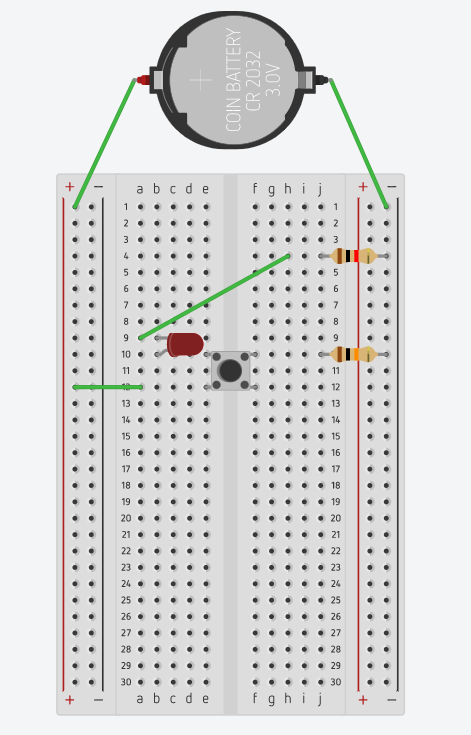
\includegraphics[width=4cm]{images/gpio-circuit.png}
	        \caption{Circuit electric}
	        \label{fig:my_label}
	    \end{figure}
        \end{minipage}
        \begin{minipage}{0.55\textwidth}\raggedleft
        \begin{itemize}
            \item \href{https://www.tinkercad.com/}{\textbf{\textit{Tinkercad}}} - platformă web utilizată în scopul proiectării și simulării unui circuit electric
        \end{itemize}
        \end{minipage}
        \noindent
        \\
	\end{frame}
	\begin{frame}
	    \frametitle{Valoarea rezistorilor}
	    \begin{itemize}
	        \item Valoarea rezistenței în Ohmi a unui rezistor se calculează pe baza numărului de benzi și a codului de culori asociat prezentat în slide-ul următor.
	        \begin{itemize}
	            \item \textit{\textbf{3 benzi}} - primele 2 dau valoarea, a 3-a multiplicator
	            \item \textit{\textbf{4 benzi}} - primele 2 dau valoarea, a 3-a multiplicator, a 4-a toleranța
	            \item \textit{\textbf{5 benzi}} - primele 3 dau valoarea, a 4-a multiplicator, a 5-a toleranța
	            \item \textit{\textbf{6 benzi}} - primele 3 dau valoarea, a 4-a multiplicator, a 5-a toleranța, a 6-a valoarea coeficientului de temperatură a materialului
	        \end{itemize}
	    \end{itemize}
	\end{frame}
	\begin{frame}
	    \frametitle{Valoarea rezistorilor}
        \begin{tabular}{|l|c|c|c|}
        \hline
        Culoare&Valoare cifră bandă&Multiplicator&Toleranță\\
        \hline
        \fcolorbox{black}{black}{\rule{0pt}{6pt}\rule{6pt}{0pt}}\quad Negru&0&x 1& - \\
        \hline
        \fcolorbox{black}{brown}{\rule{0pt}{6pt}\rule{6pt}{0pt}}\quad Maro&1&x 10& \pm 1\% \\
        \hline
        \fcolorbox{black}{red}{\rule{0pt}{6pt}\rule{6pt}{0pt}}\quad Roșu&2&x 10^2& \pm 2\% \\
        \hline
        \fcolorbox{black}{orange}{\rule{0pt}{6pt}\rule{6pt}{0pt}}\quad Portocaliu&3&x 10^3& \pm 0.05\% \\
        \hline
        \fcolorbox{black}{yellow}{\rule{0pt}{6pt}\rule{6pt}{0pt}}\quad Galben&4&x 10^4& \pm 0.02\% \\
        \hline
        \fcolorbox{black}{green}{\rule{0pt}{6pt}\rule{6pt}{0pt}}\quad Verde&5&x 10^5& \pm 0.5\% \\
        \hline
        \fcolorbox{black}{blue}{\rule{0pt}{6pt}\rule{6pt}{0pt}}\quad Albastru&6&x 10^6& \pm 0.25\% \\
        \hline
        \fcolorbox{black}{violet}{\rule{0pt}{6pt}\rule{6pt}{0pt}}\quad Violet&7&x 10^7& \pm 0.1\% \\
        \hline
        \fcolorbox{black}{gray}{\rule{0pt}{6pt}\rule{6pt}{0pt}}\quad Gri&8&x 10^8& \pm 0.01\% \\
        \hline
        \fcolorbox{black}{white}{\rule{0pt}{6pt}\rule{6pt}{0pt}}\quad Alb&9&x 10^9& - \\
        \hline
        \fcolorbox{black}{gold}{\rule{0pt}{6pt}\rule{6pt}{0pt}}\quad Auriu&-&x 0.1& \pm 5\% \\
        \hline
        \fcolorbox{black}{silver}{\rule{0pt}{6pt}\rule{6pt}{0pt}}\quad Argintiu&-&x 0.01& \pm 10\% \\
        \hline
        \end{tabular}
	\end{frame}
	\section{Configurare}
	\begin{frame}
	    \frametitle{\href{https://github.com/undacmic/MCULabs/blob/main/Resurse/FRDM-KL25Z_ReferenceManual.pdf}{Setarea regiștrilor}}
	    \begin{itemize}
	        \item Dacă un pin are funcția de GPIO, atunci vom putea să îi controlăm direcția și valoarea în mod programatic. Vom realiza acest lucru prin scrieri/citiri în/din registre speciale, ce controlează exact acest comportament.
	        \item Registrele care controlează comportamentul unui port sunt:
	        \begin{itemize}
	            \item \textbf{\textit{GPIOx\_PDDR}} - Port Data Direction Register
	            \item \textbf{\textit{GPIOx\_PDIR}} - Port Data Input Register
	            \item \textbf{\textit{GPIOx\_PDOR}} - Port Data Output Register
	            \item \textbf{\textit{GPIOx\_PSOR}} - Port Set Output Register
	            \item \textbf{\textit{GPIOx\_PCOR}} - Port Clear Output Register
	            \item \textbf{\textit{GPIOx\_PTOR}} - Port Toggle Output Register
	        \end{itemize}
	    \end{itemize}
	\end{frame}
		\begin{frame}
	    \frametitle{\href{https://github.com/undacmic/MCULabs/blob/main/Resurse/FRDM-KL25Z_ReferenceManual.pdf}{Setarea regiștrilor}}
	    \begin{itemize}
	        \item Activarea semnalului de ceas pentru a putea configura modulele folosite
	        \begin{itemize}
	            \item \textbf{\textit{SIM\_SCGC5}} - portul de pe care vom configura pinii folosiți pentru I/O
	        \end{itemize}
	        \item \textbf{\textit{PORTx\_PCR}} - multiplexarea semnalului pe pini (\textbf{\textit{MUX}}) și configurarea nivelului pe care se va primi întreruperea \textbf{(rising/falling edge - \textit{IRQC})}
	        \item \textbf{\textit{GPIOx\_PDDR}} - configurarea pinului pentru intrare (\textbf{0}) sau ieșire (\textbf{1})
	        \item \textbf{\textit{GPIOx\_PCOR, GPIOx\_PSOR și GPIOx\_PTOR}} - manipularea nivelului logic de pe pinul de ieșire
	    \end{itemize}
	\end{frame}
	\section{Exemplu practic}
	\begin{frame}
	    \frametitle{Experiment}
	    \begin{itemize}
	        \item Componente utilizate
	        \begin{itemize}
	            \item \textbf{\textit{Switch}} - \textbf{\textit{PTA12}}
	            \item \textbf{\textit{Aranjament de tipul pull-down}}
	            \item \textbf{\textit{	    \href{https://github.com/undacmic/MCULabs/blob/main/Resurse/FRDM-KL25Z_Schematics.pdf}{LED RGB}}} disponibil pe plăcuță, astfel:
	            \begin{itemize}
	                \item \color{red} RED LED - \textbf{PTB18}
	                \item \color{green} GREEN LED - \textbf{PTB19}
	                \item \color{blue} BLUE LED - \textbf{PTD1}
	            \end{itemize}
	        \end{itemize}
	    \end{itemize}
	    \begin{figure}
	        \centering
	        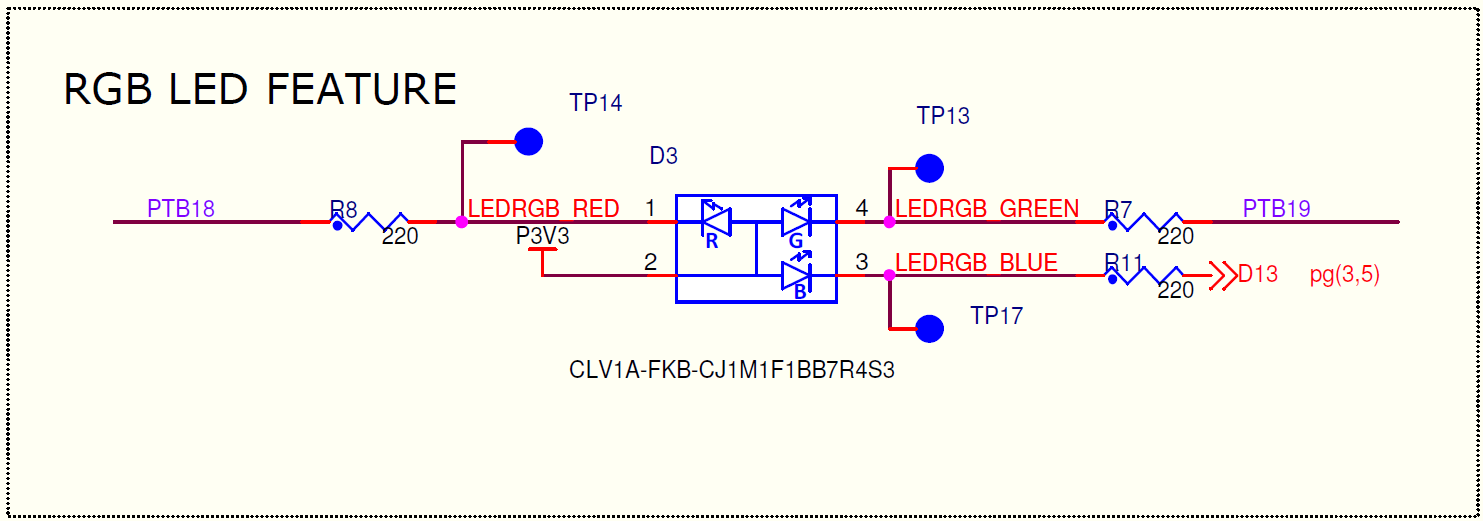
\includegraphics[width=7.5cm]{images/rgb-led.png}
	        \caption{RGB LED Schematic}
	        \label{fig:my_label}
	    \end{figure}
	\end{frame}
	\begin{frame}
	    \frametitle{Experiment}
	    \begin{figure}
	        \centering
	        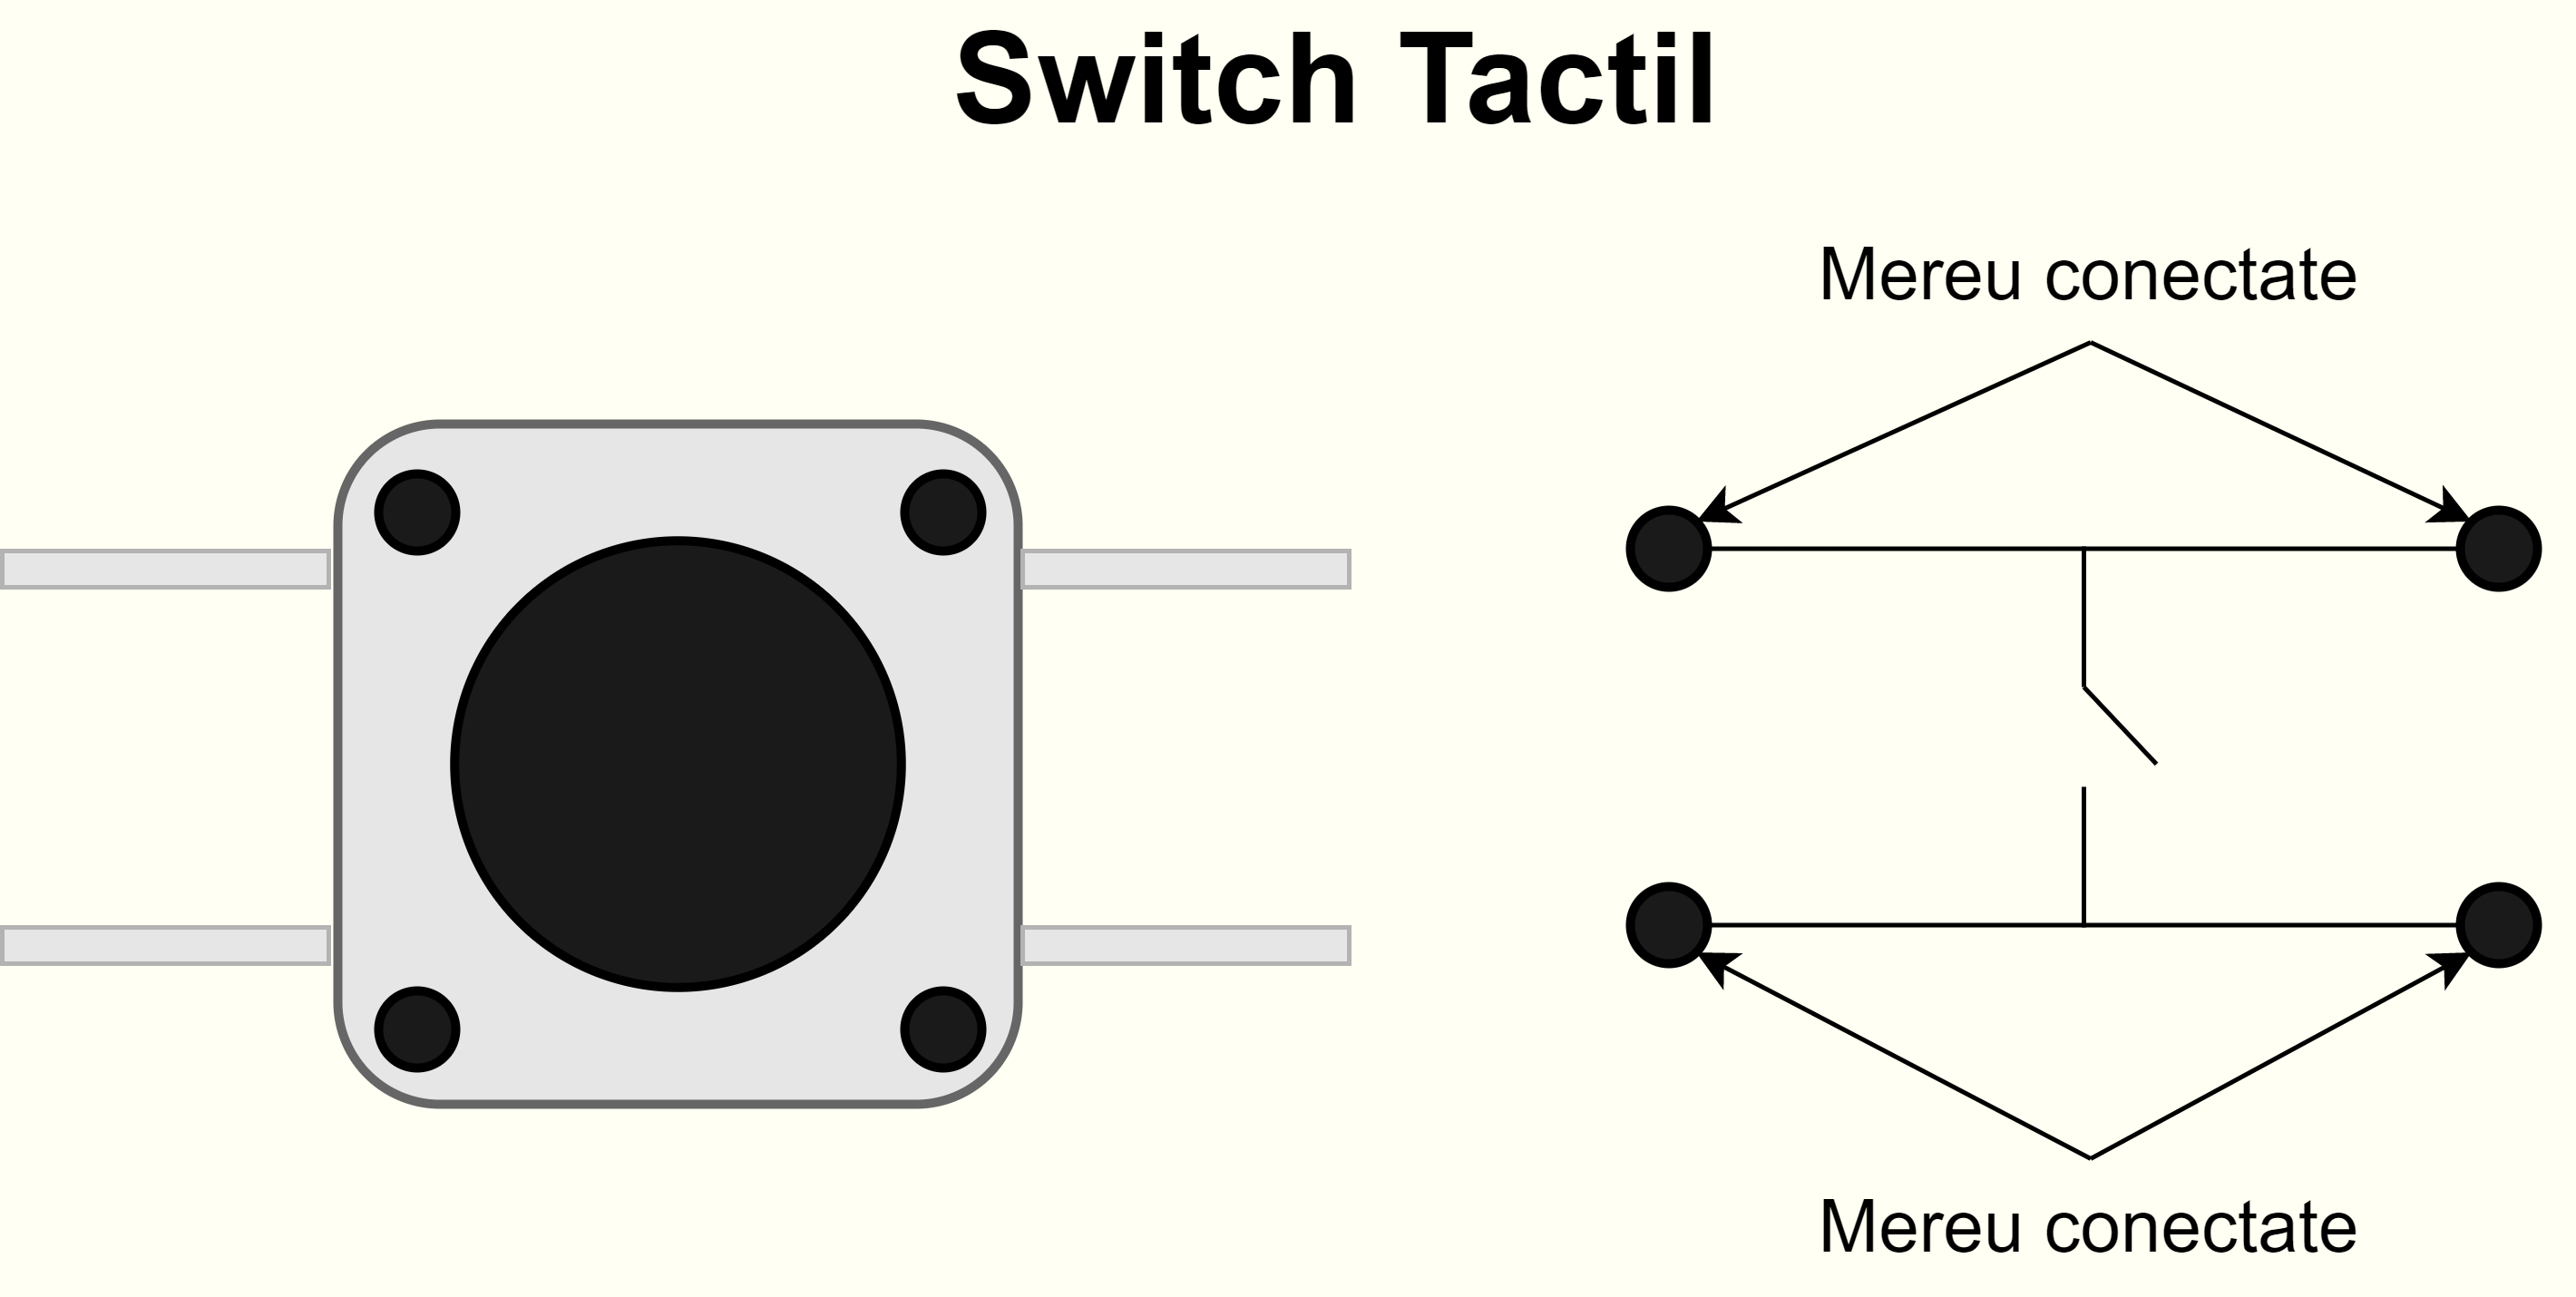
\includegraphics[width=9cm]{images/switch-diagrama.png}
	        \caption{Diagrama unui switch tactil}
	        \label{fig:my_label}
	    \end{figure}
	\end{frame}
	\begin{frame}
	    \frametitle{Experiment}
	    \begin{itemize}
	        \item Întrucât led-urile sunt conectate la 3.3V, va trebui setată valoarea logică 0 pe pinii respectivi, pentru ca diferența de tensiune să fie una pozitivă și led-urile să se aprindă
	        \item \textbf{\textit{Obiectiv: }} Prin apăsarea switch-ului, să aprindem pe rând cele trei led-uri componente
	        \item Avem nevoie de activarea înteruperilor pe portul A și suprascrierea handler-ului de întreruperi \textbf{\textit{PORTA\_IRQHandler}}
	        \item Realizarea conexiunilor cu \textbf{VCC} și \textbf{GND}
	    \end{itemize}
	\end{frame}
		\begin{frame}
	    \frametitle{Rezultat}
	    \begin{figure}
	        \centering
	        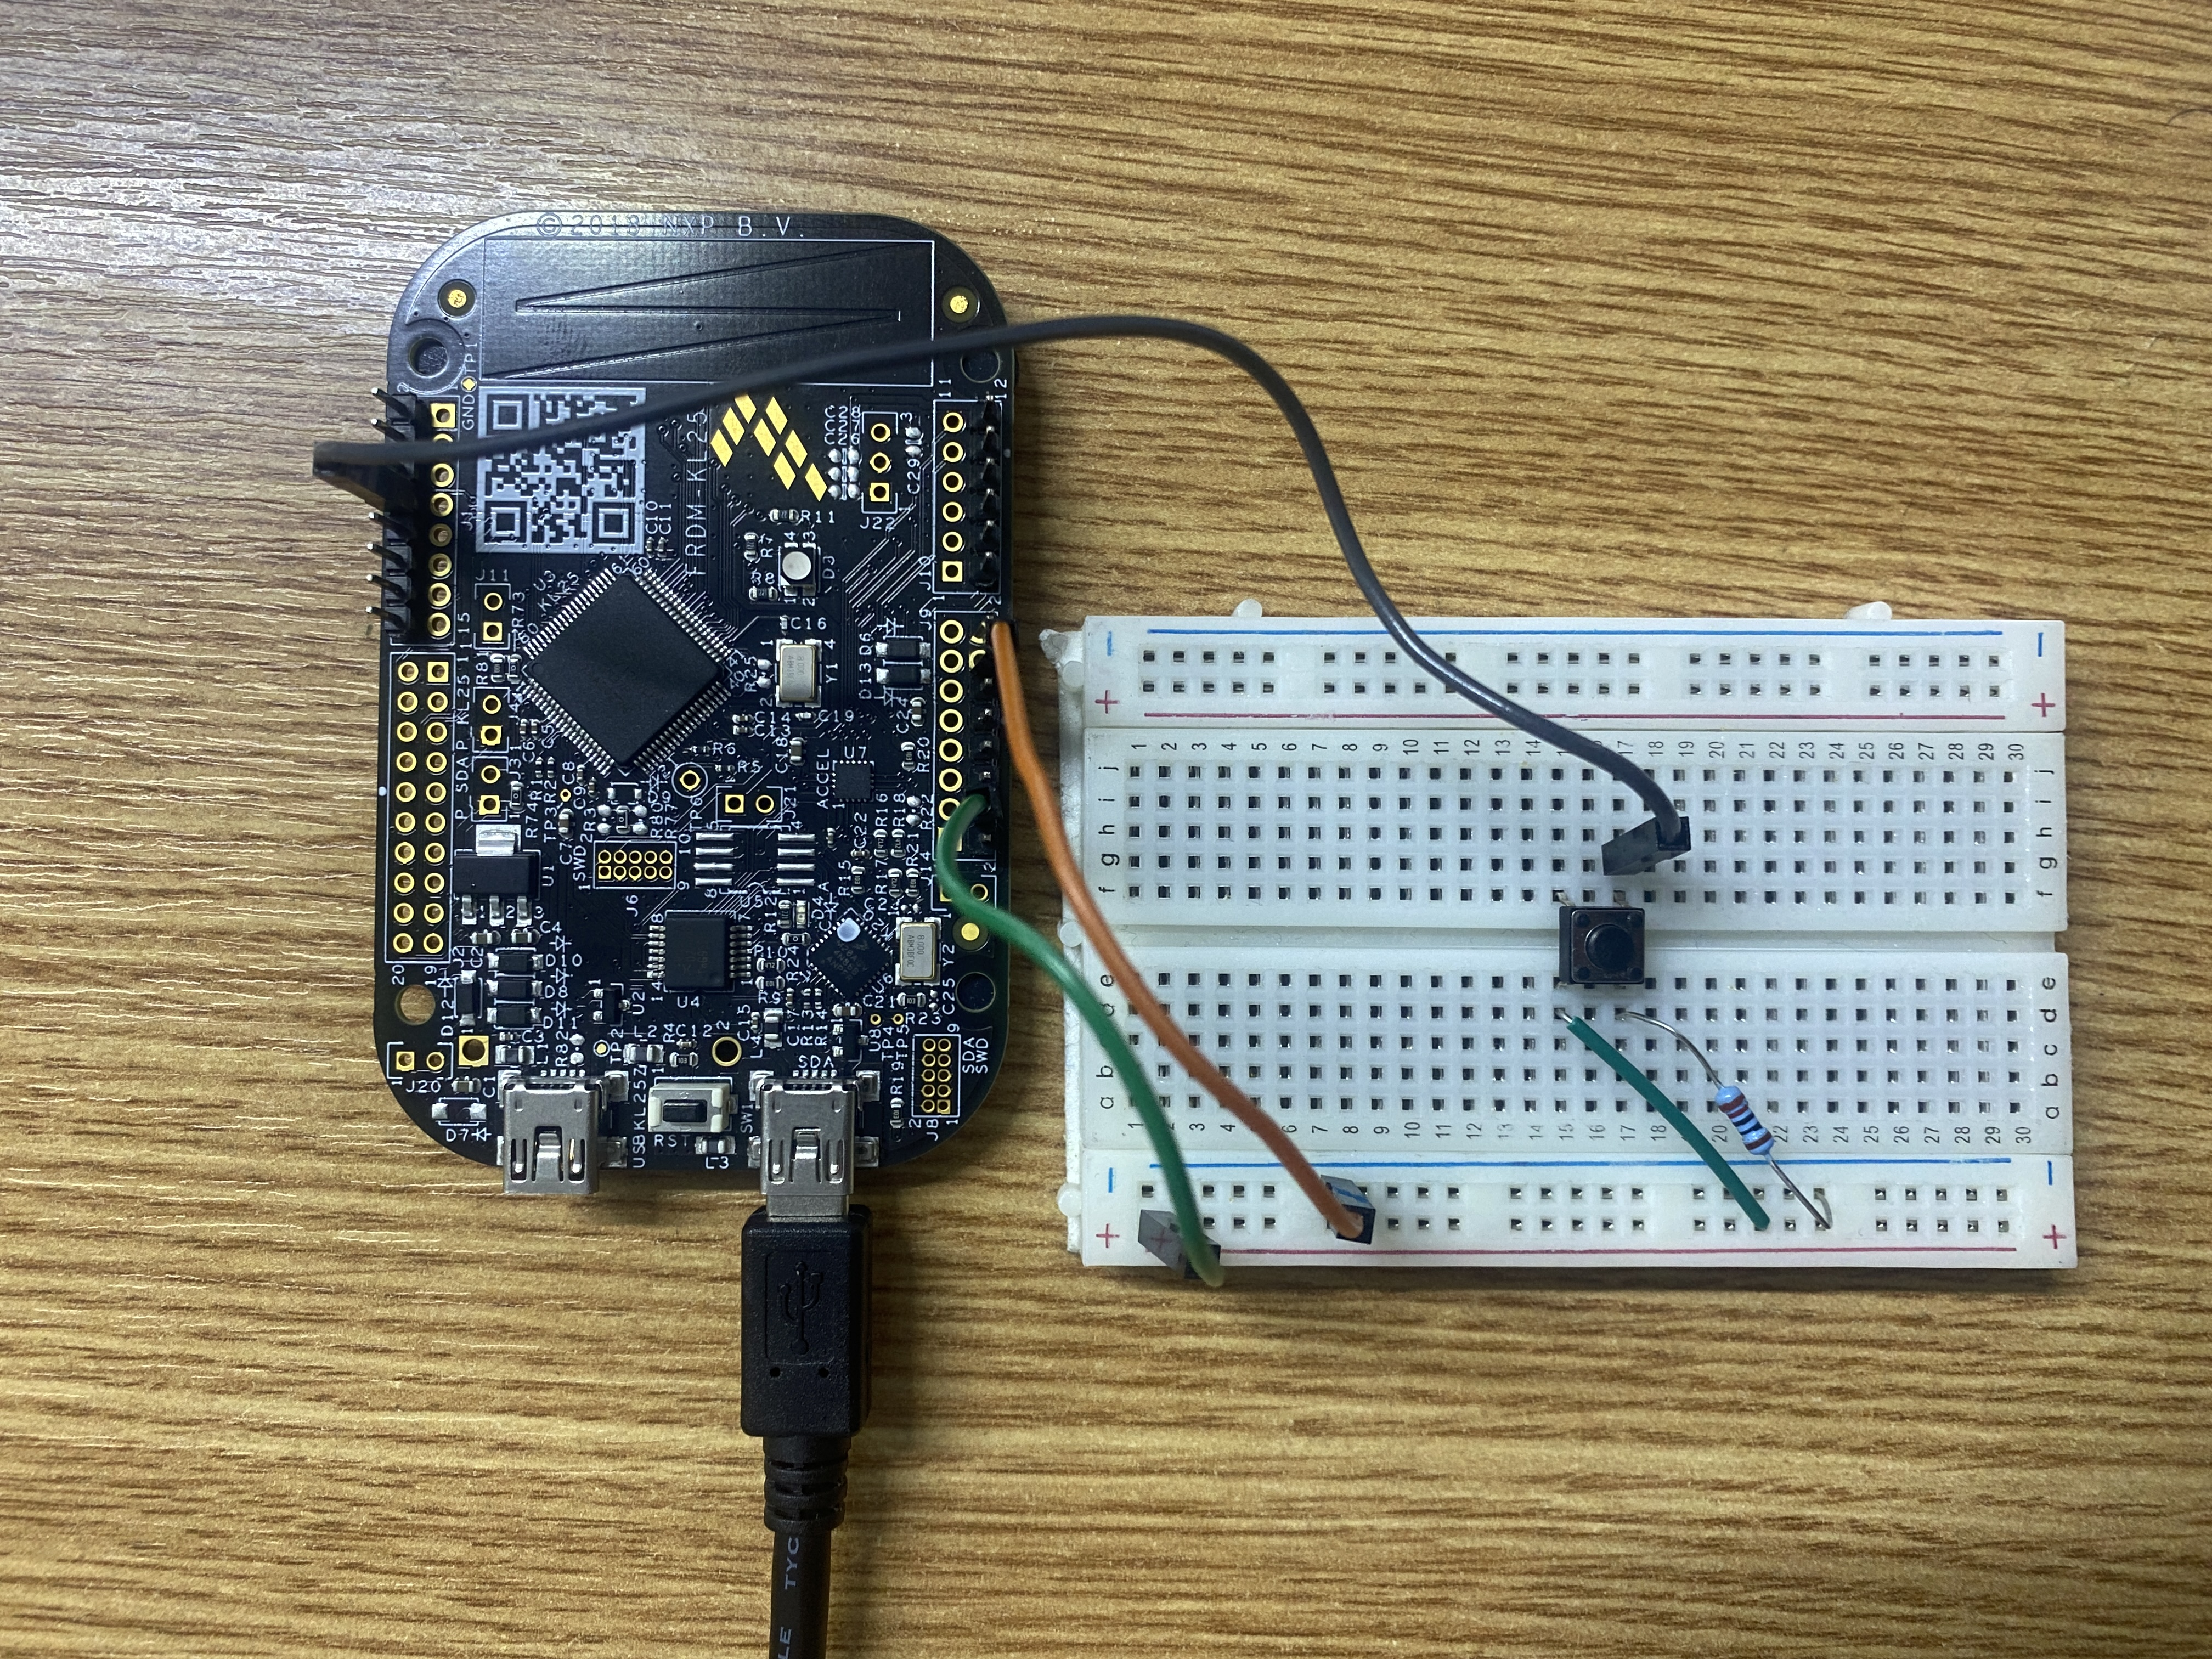
\includegraphics[width=8cm]{images/Ansamblu.jpg}
	        \caption{Circuit electric final}
	        \label{fig:my_label}
	    \end{figure}
	\end{frame}
	\appendix


\end{document}